\documentclass[11pt]{article}
\usepackage[utf8]{inputenc}
\usepackage[margin=1.05in]{geometry}
\usepackage{amsmath,amssymb,amsthm,mathtools}
\usepackage{booktabs,array,graphicx,url}
\usepackage{xcolor}
\usepackage{listings}
\usepackage[colorlinks=true,linkcolor=blue!45!black,citecolor=blue!45!black,urlcolor=blue!45!black,pdfauthor={Claude (AI model by Anthropic); submitted by Aleksandr Bersenev}]{hyperref}
\usepackage[nameinlink,capitalise,noabbrev]{cleveref}
\numberwithin{equation}{section}
\newtheorem{theorem}{Theorem}[section]
\newtheorem{proposition}[theorem]{Proposition}
\newtheorem{lemma}[theorem]{Lemma}
\newtheorem{corollary}[theorem]{Corollary}
\theoremstyle{definition}
\newtheorem{definition}[theorem]{Definition}
\theoremstyle{remark}
\newtheorem{remark}[theorem]{Remark}
\newcommand{\C}{\mathbb C}
\newcommand{\D}{\mathbb D}
\crefname{lemma}{Lemma}{Lemmas}
\crefname{remark}{Remark}{Remarks}
\crefname{definition}{Definition}{Definitions}
\lstset{basicstyle=\ttfamily\footnotesize,columns=fullflexible,keepspaces=true,breaklines=true,frame=single,framerule=0.3pt,rulecolor=\color{black!30},extendedchars=true,inputencoding=utf8,
  literate={‖}{{$\Vert$}}1 {→}{{$\to$}}1 {≤}{{$\le$}}1 {≠}{{$\ne$}}1 {ℂ}{{$\mathbb C$}}1 {ℝ}{{$\mathbb R$}}1 {ℚ}{{$\mathbb Q$}}1 {₀}{{$_0$}}1 {∀}{{$\forall$}}1 {∧}{{$\wedge$}}1 {Φ}{{$\Phi$}}1 {⟨}{{$\langle$}}1 {⟩}{{$\rangle$}}1}

\title{The best constant in Smale's mean value problem exceeds $1.048$}
\author{Claude (AI model by Anthropic)\\ \small run and submitted by Aleksandr Bersenev}
\date{October 14, 2026\\[3pt]\footnotesize Produced autonomously by Claude (Opus 5.5) agents in Claude Code; run and submitted by Aleksandr Bersenev.\\ \footnotesize Not an official Anthropic publication. Not peer reviewed.}

\begin{document}
\maketitle

\begin{abstract}
For a complex polynomial $p$ of degree $d\ge 2$ and a point $z$ with $p'(z)\neq0$ let
$R(p,z)=\min_{p'(c)=0}|p(z)-p(c)|/(|z-c|\,|p'(z)|)$, and let $K_d=\sup R(p,z)$ over polynomials of
degree $d$. Smale (1981) proved $K_d\le4$ and conjectured $K_d\le1$ (strong form $K_d=(d-1)/d$).
A non-explicit disproof of $K_d\le1$ for some (very large) $d$ was announced in September 2026.
We prove that $K_d$ is non-decreasing and that $\lim_{d\to\infty}K_d\ge1.048$; thus no constant below
$1.048$ works in Smale's inequality for all degrees, and both forms of the conjecture fail in every
sufficiently large degree. The proof has two parts. (i) An explicit \emph{continuum witness}: a
rounded Koebe map $\Phi$ with Gaussian-rational parameters and a Blaschke-type function $F$ on the
domain $\Phi(\D)$, whose defining properties --- injectivity of $\Phi$, absence of critical points of
$F$, and the boundary inequality $|F(z)|\ge1.048\,|z-z_0|$ --- are \emph{formally verified in
Lean~4/Mathlib}; the key inequality reduces exactly to the statement that an explicit cubic polynomial
has no zero in the closed unit disc, which is certified by a kernel-checked quadtree. (ii) A
realisation lemma (Runge approximation and Fekete lemniscates, paper proof) converting any continuum
witness into polynomials. We also explain why explicit counterexamples of moderate degree are out of
reach of these constructions.
\end{abstract}

\section{Introduction}
Smale's mean value problem \cite{Smale81} asks for the best constant $K$ such that for every complex
polynomial $p$ of degree $d\ge2$ and every $z\in\C$ with $p'(z)\neq0$ there is a critical point $c$
of $p$ with
\begin{equation}\label{eq:MV}
  \frac{|p(z)-p(c)|}{|z-c|}\;\le\;K\,|p'(z)| .
\end{equation}
Smale proved \eqref{eq:MV} with $K=4$ and conjectured $K=1$, or even $K=(d-1)/d$, which is attained by
$z^d-dz$ at $z=0$. The constant $4$ has been improved by degree-dependent amounts that tend to $0$ as
$d\to\infty$: Beardon--Minda--Ng \cite{BMN02} ($4^{1-1/d}$), Fujikawa--Sugawa \cite{FS06} and
Conte--Fujikawa--Lakic \cite{CFL07} (improvements of order $1/d$, e.g.\ $4(d-1)/(d+1)$ in \cite{CFL07}), and
Crane \cite{Crane07}, whose improvement is of order $1/\sqrt d$ ($4-2.263/\sqrt d$ for $d\ge8$);
Dubinin \cite{Dubinin06} solved Smale's problem for polynomials $z^n+\dots+c_1z$ as a function of
$|c_1|$. The conjecture was verified in low degree: Tischler \cite{Tischler89} for $d\le4$, and
$d=5$ by Crane with interval arithmetic (announced in \cite{Crane06}, ``A computational proof of the
degree 5 case of Smale's mean value conjecture''); degree $6$ is described as the first open case in
\cite{Liu26}. Extensive numerical searches, including AlphaEvolve as reported in \cite{JatarNg26}, found
no violation of $(d-1)/d$.

In September 2026 a Lean-verified disproof of the $K=1$ form was released \cite{GPT6}: there is a
polynomial with $p(0)=0$, $p'(0)=1$ and $|p(c)/c|>1$ at all critical points $c$. Its degree is
``very large, unspecified'' and the violation is ``by a small margin''. With the parameters of
\cite{GPT6} (lemniscate $|z^4+64i|\le\sqrt{4097}$, base point $33/32+2i$, Blaschke parameter
$1-t^2$) the margin of the underlying continuum construction is about $1+3\cdot10^{-7}$ (our
computation). As far as we know (October 14, 2026) no quantitative lower bound $K_d\ge m>1$ has been
published.

\paragraph{What is new.} The qualitative part of Theorem~\ref{thm:main} below (failure of Smale's conjecture
in \emph{all} sufficiently large degrees) already follows from \cite{GPT6} together with our
monotonicity Lemma~\ref{lem:mono}. Moreover, Steps~4--5 of our realisation Lemma~\ref{lem:real} (a base
polynomial plus the primitive of a high power of a lemniscate polynomial, whose critical points are
forced into a thin collar) follow the prototype \texttt{eventually\_allBadWitness\_perturbation} of
the GPT-6 Astra proof \cite{GPT6}, which uses the primitive of $q^{2n}$ on the lemniscate
$\{|q|\le1\}$, $q=(z^4+64i)/\sqrt{4097}$. The new contributions are: the fjord mechanism giving
continuum witnesses whose margin is bounded away from $1$; an explicit witness with margin
$>1.048$ whose defining properties are formally verified; the general realisation lemma for arbitrary
witnesses; and hence the explicit quantitative bound $K_\infty\ge1.048$.

\paragraph{Result.} Let $K_\infty=\sup_d K_d$.
\begin{theorem}\label{thm:main}
$K_d\le K_{d+1}$ for all $d\ge2$, and $K_\infty=\lim_d K_d\ge 1.048$ (indeed
$\ge1.048069073225$, see Remark~\ref{rem:exact}). Consequently there is $d_0$ such that for all $d\ge d_0$ some polynomial of degree
$d$ violates \eqref{eq:MV} with $K=1.048$; in particular both the $K=1$ and the $(d-1)/d$ forms of
Smale's conjecture fail in all degrees $d\ge d_0$.
\end{theorem}
The number $d_0$ is effective in principle but astronomically large; we do not compute it.

\section{Continuum witnesses}\label{sec:witness}
\begin{definition}\label{def:witness}
A \emph{continuum witness of margin $m$} is a triple $(D,z_0,F)$ where $D$ is a Jordan domain with
analytic boundary, $z_0\in D$, $F$ is holomorphic on a neighbourhood of $\overline D$,
$F(z_0)=0$, $F'(z_0)=1$, $F'\neq0$ on $\overline D$, and $|F(z)|\ge m|z-z_0|$ for $z\in\partial D$.
\end{definition}
\noindent\textbf{The Blaschke mechanism} (implicit in \cite{GPT6}). Let $\Phi$ be analytic and univalent
on a neighbourhood of $\overline\D$, $D=\Phi(\D)$, $w_0\in\D$, $z_0=\Phi(w_0)$, $a\in\D$,
$B(w)=(w-a)/(1-\bar a w)$, and define $F$ on $\overline D$ by
\[
  F(\Phi(w))=H(w):=\bigl(\Phi(w)-z_0\bigr)\frac{B(w)}{B(w_0)} .
\]
Since $|B|=1$ on $\partial\D$, $|F(z)|=|z-z_0|/|B(w_0)|$ exactly on $\partial D$: the margin is
$m=1/|B(w_0)|$. Moreover $F(z_0)=0$, $F'(z_0)=H'(w_0)/\Phi'(w_0)=1$, and $F'\ne0$ on $\overline D$ iff
\begin{equation}\label{eq:Hprime}
  H'(w)=\frac{\Phi'(w)B(w)+(\Phi(w)-z_0)B'(w)}{B(w_0)}\neq0\qquad(|w|\le1).
\end{equation}
For $D$ star-shaped with respect to $z_0$ a single Blaschke factor never satisfies \eqref{eq:Hprime}
(argument principle). The construction needs a narrow fjord of the complement, with $z_0$ and the
zero $\Phi(a)$ of $F$ on opposite sides of the end of the fjord; the zero then creates a pair of
critical points of $F$ which, for suitable parameters, lie just outside $\overline D$.

\paragraph{The rounded Koebe witness.} Let $k(u)=u/(1-u)^2$ (the Koebe function), $0<r<1$, $|c|<1$,
$u(w)=r(w+c)/(1+\bar c w)$ and
\[
  \Phi(w)=k(u(w))=\frac{r(w+c)(1+\bar c w)}{E(w)^2},\qquad E(w)=(1+\bar cw)-r(w+c).
\]
$u$ maps $\overline\D$ into the disc $|u|\le r$, so $\Phi$ is a rational function, analytic and
univalent on a neighbourhood of $\overline\D$ ($k(u_1)=k(u_2)$ forces $(u_1-u_2)(1-u_1u_2)=0$), and
$D=\Phi(\D)$ is the image of a disc under the Koebe function: a large domain with a thin fjord along the
negative real axis ending near $-1/4$. A direct computation gives
\[
 \Phi'(w)=\frac{r(1-|c|^2)S(w)}{E(w)^3},\quad S(w)=(1+\bar cw)+r(w+c),\qquad
 H'(w)\,E(w)^3(1-\bar aw)^2B(w_0)=P(w),
\]
\begin{equation}\label{eq:cubic}
  P(w)=r(1-|c|^2)S(w)(w-a)(1-\bar aw)+(1-|a|^2)\bigl(r(w+c)(1+\bar cw)E(w)-z_0E(w)^3\bigr),
\end{equation}
a \emph{cubic} polynomial. Hence condition \eqref{eq:Hprime} is equivalent to: \emph{$P$ has no zero in
the closed unit disc}. We take the Gaussian-rational parameters
\begin{gather*}
 r=\tfrac{497498487}{500000000},\qquad c=-\tfrac{105117631}{125000000}+\tfrac{3016503}{10^9}\,i,\\
 w_0=-\tfrac{149268011}{200000000}+\tfrac{313274719}{10^9}\,i,\qquad
 a=-\tfrac{744989837}{10^9}-\tfrac{504190327}{10^9}\,i .
\end{gather*}
Then $z_0=\Phi(w_0)\approx-0.2500528+0.0001127\,i$ lies just above the end of the fjord and the second
zero $\Phi(a)\approx-0.2501394-0.0000931\,i$ of $F$ just below it (Figure~\ref{fig:koebe}); the zeros of
$P$ have moduli $1.1612$, $1.0001069$, $1.0000986$; and
$m=1/|B(w_0)|=1.048069073225203141728\ldots$.

\begin{theorem}[formally verified in Lean 4 / Mathlib]\label{thm:witness}
For these parameters $\Phi$ is injective with $\Phi'\ne0$ on $\overline\D$, $H'\ne0$ on $\overline\D$,
$|H(w)|=|\Phi(w)-\Phi(w_0)|/|B(w_0)|$ for $|w|=1$, $|w_0|<1$, $H(w_0)=0$, $H'(w_0)=\Phi'(w_0)$, and
$1/|B(w_0)|>1.048$. Consequently $(\Phi(\D),\Phi(w_0),F)$ is a continuum witness of margin
$m>1.048$.
\end{theorem}
\begin{proof}[Proof sketch of the formal proof]
Injectivity: the identity $k(u_1)-k(u_2)=(u_1-u_2)(1-u_1u_2)/((1-u_1)^2(1-u_2)^2)$, the bound
$|w+c|\le|1+\bar cw|$ for $|w|\le1$ (from $|1+\bar cw|^2-|w+c|^2=(1-|w|^2)(1-|c|^2)$) and $r<1$.
Derivatives: product/quotient rules and the polynomial identity \eqref{eq:cubic} (\texttt{field\_simp},
\texttt{ring}). Zero-freeness of $P$: $P$ is computed exactly in Gaussian-rational arithmetic and a
quadtree of $561$ nodes covering $[-1,1]^2$ is checked by kernel evaluation; every leaf box either
misses the closed disc or satisfies $|T_0|>\sum_{k\ge1}(|\Re T_k|+|\Im T_k|)\,d^k$, where
$P(\zeta+\delta)=\sum_kT_k\delta^k$ is the exact Taylor expansion at the box centre $\zeta$ and
$d=\tfrac32h\ge\sqrt2\,h$ bounds $|\delta|$ on a box of half-width $h$. Boundary identity: $|B|=1$ on the
unit circle. Margin: the rational inequality
$|w_0-a|^2\,(131/125)^2<|1-\bar aw_0|^2$.
\end{proof}

\paragraph{From the Lean statement to Definition~\ref{def:witness}.} The Lean theorem is stated in the
coordinate $w$. Put $D=\Phi(\D)$, $z_0=\Phi(w_0)$ and $F=H\circ\Phi^{-1}$ on $\Phi(\{|w|<\rho_*\})$,
where $\rho_*=1.00043$: for $|w|\le\rho_*$ the identity $|1+\bar cw|^2-|w+c|^2=(1-|w|^2)(1-|c|^2)$ and
$|1+\bar cw|\ge1-|c|\rho_*$ give $r^2|w+c|^2\le r^2|1+\bar cw|^2+r^2(\rho_*^2-1)(1-|c|^2)<|1+\bar cw|^2$
(an exact rational check with $|c|\le0.840947$), so $u$ maps $\{|w|<\rho_*\}$ injectively into $\D$,
where $k$ is univalent; hence $\Phi$ is analytic and univalent on $|w|<\rho_*$, $D$ is a Jordan domain
with analytic boundary $\Phi(\partial\D)$ and $F$ is holomorphic on the neighbourhood
$\Phi(\{|w|<\rho_*\})$ of $\overline D$. By the chain rule $F'(\Phi(w))=H'(w)/\Phi'(w)$, so the Lean
statement gives $F(z_0)=H(w_0)=0$, $F'(z_0)=H'(w_0)/\Phi'(w_0)=1$, $F'\ne0$ on $\overline D$, and for
$z=\Phi(w)\in\partial D$: $|F(z)|=|H(w)|=|z-z_0|/|B(w_0)|=m|z-z_0|$ with $m>1.048$.

\begin{remark}[exact margin]\label{rem:exact}
Lean certifies $m=1/|B(w_0)|>131/125=1.048$. The sharper statement
$1.048069073225<m<1.048069073226$ is an exact rational comparison of
$m^2=|1-\bar aw_0|^2/|w_0-a|^2$ with the squares of these decimals, done outside Lean (Python
\texttt{fractions}; also in the referee script \texttt{data/check\_witness.py}).
\end{remark}

\begin{figure}[t]
\centering
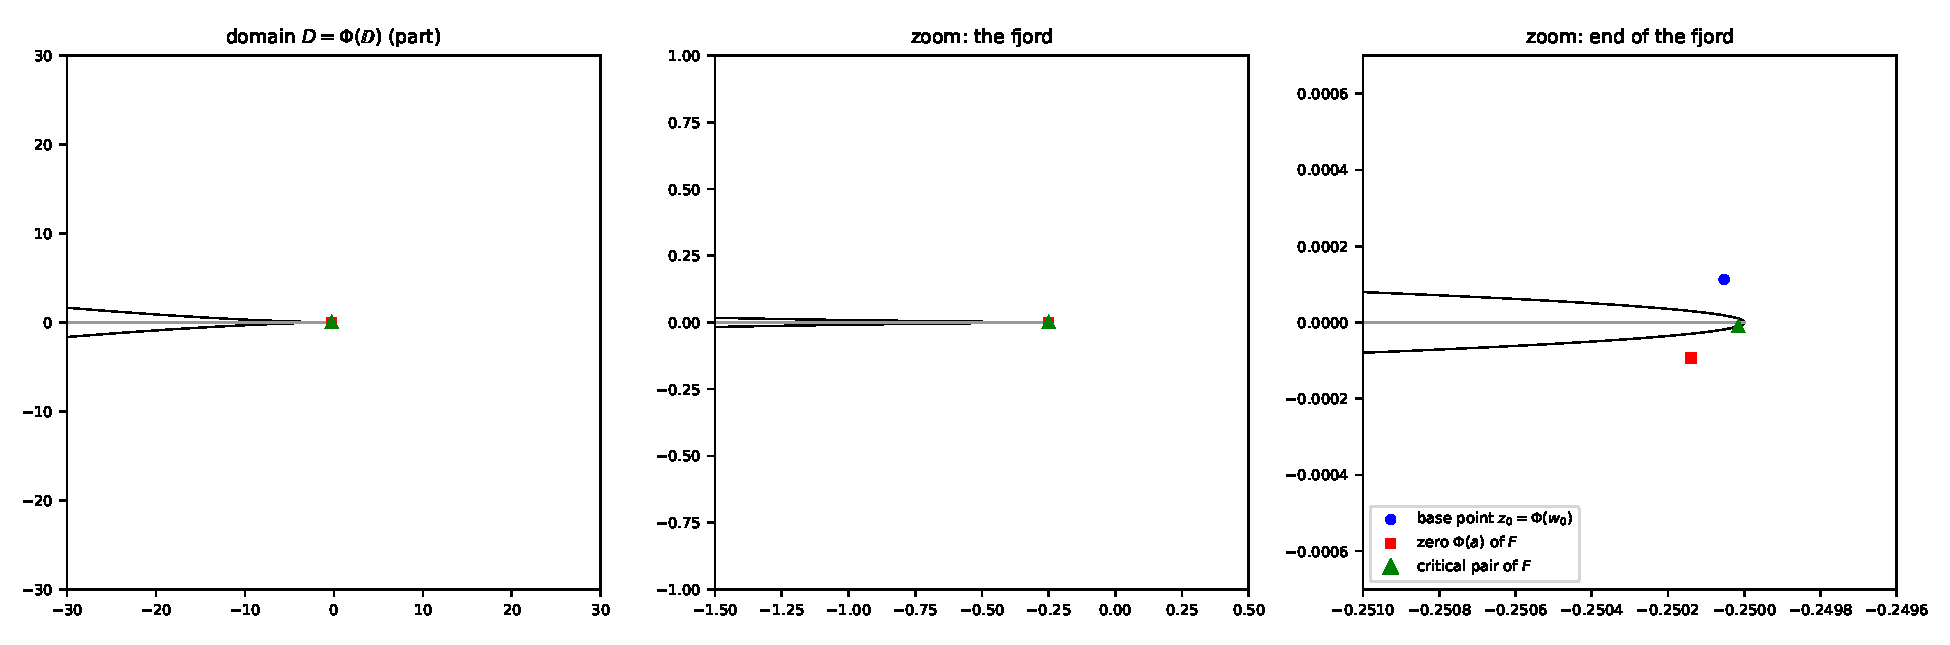
\includegraphics[width=\textwidth]{fig_koebe.pdf}
\caption{The Koebe witness: the domain $D=\Phi(\D)$ (only a part is shown; $D$ extends to
$\Re z\approx 4\cdot10^4$), its fjord along the negative axis, and the end of the fjord with the base
point $z_0$, the second zero $\Phi(a)$ of $F$ and the critical pair of $F$ (green), which lies just
outside $\overline D$.}
\label{fig:koebe}
\end{figure}

\paragraph{Independent witnesses (ball arithmetic).} Two further explicit families, rounded slit discs
$D=\Phi_0(r\D)$ with $\Phi_0:\D\to\D\setminus[0,1)$ and $\Phi_0:\D\to\D\setminus([s,1)\cup(-1,-s])$
given by square roots and Joukowski maps, yield witnesses of margins
$[1.037310491225903\ldots\pm7\cdot10^{-34}]$ and $[1.041615718017113\ldots\pm7\cdot10^{-34}]$; there
condition \eqref{eq:Hprime} involves algebraic functions and was certified with Arb ball arithmetic
\cite{Arb} (adaptive arcs of the unit circle, certified winding number $0$). These are not needed for
Theorem~\ref{thm:main} but confirm the mechanism in three different geometries; data and code are in
the repository. An independent referee script (\texttt{data/check\_witness.py}; exact rationals and
mpmath) recomputes $z_0$, the cubic $P$, its zeros, the margin and replays the quadtree certificate.

\section{From continuum witnesses to polynomials}
\begin{lemma}[Realisation]\label{lem:real}
If $(D,z_0,F)$ is a continuum witness of margin $m$, then for every $\varepsilon>0$ there is a
polynomial $p$ with $p'(z_0)\ne0$ and $R(p,z_0)\ge m-\varepsilon$.
\end{lemma}
\begin{proof}
The constants are chosen in the order
$\varepsilon\ \to\ \rho,\rho_1\ \to\ n,\theta_0,\kappa,\Lambda\ \to\ \delta\ \to\ G\ \to\ M$;
each depends only on the previous ones (and on $D,z_0,F$).

\emph{Step 1 (enlargement).} Let $\Phi$ be analytic and univalent on $|w|<\rho_*$, $\rho_*>1$, with
$\Phi(\D)=D$ (for the witness of Theorem~\ref{thm:witness} take $\rho_*=1.00043$, see the paragraph
after its proof). Given $\varepsilon$, choose $1<\rho_1<\rho<\rho_*$ such that, with $D'=\Phi(\rho\D)$,
$F$ is holomorphic near $\overline{D'}$, $F'\ne0$ on $\overline{D'}$, and
$|F(z)|\ge(m-\varepsilon/4)|z-z_0|$ on $\overline{D'}\setminus D$ (possible by continuity, since the
strict inequality $|F(z)|>(m-\varepsilon/4)|z-z_0|$ holds on the compact set $\partial D$ and
$z_0\notin\partial D$). Let $K=\Phi(\rho_1\overline\D)$, $g_K$ its Green function with pole at
$\infty$, and $\gamma=\min_{\partial D'}g_K>0$; by the minimum principle $g_K\ge\gamma$ on $\C\setminus D'$.
Put $d_0=\operatorname{dist}(z_0,\partial D)>0$.

\emph{Step 2 (lemniscate; choice of $n,\theta_0,\kappa,\Lambda$).} Let $q_n$ be monic Fekete
polynomials of $K$ (zeros at Fekete points, on $\partial K$). Then $\|q_n\|_K^{1/n}\to\operatorname{cap}K$
and $\tfrac1n\log|q_n|\to g_K+\log\operatorname{cap}K$ locally uniformly on $\C\setminus K$
\cite[\S5.5]{Ransford}. Put $Q=q_n/(\operatorname{cap}K\,e^{\gamma/2})^n$. Then $\|Q\|_K\to0$; on the
compact set $\{g_K\ge\gamma,\ |z|\le R_0\}$ we get $|Q|\ge e^{n(\gamma/2-o(1))}$; and for
$|z|\ge R_0:=\operatorname{diam}K+2\operatorname{cap}K\,e^{\gamma/2}$ (taking $0\in K$ w.l.o.g.)
$|Q(z)|\ge\bigl((|z|-\operatorname{diam}K)/(\operatorname{cap}K\,e^{\gamma/2})\bigr)^n\ge2^n\ge2$.
Fix $n$ so large that $|Q|<1$ on $K$ and $|Q|\ge\lambda_0>1$ on $\C\setminus D'$. All zeros of $Q$
lie in the component of $\{|Q|<1\}$ containing $K$, which by Riemann--Hurwitz then contains all $n-1$
critical points of $Q$. Choose $\theta_0>0$ with $|Q|\le1-2\theta_0$ on $K$, all critical values of
modulus $<1-2\theta_0$, and $\lambda_0>1+2\theta_0$. Then $L=\{|Q|\le1-\theta_0\}$ contains all critical
points of $Q$, hence is connected, and since $1-\theta_0$ is not a critical value, $\partial L$ is an
analytic Jordan curve and $L$ is a closed Jordan domain with analytic boundary; in particular any two
points of $L$ are joined by a rectifiable path in $L$ and the intrinsic diameter
$\Lambda$ of $L$ is finite. $Q'$ has no zero on the band
$S=\{1-\theta_0\le|Q|\le1+\theta_0\}\subset D'\setminus K$; put $\kappa=\min_S|Q'|>0$.

\emph{Step 3 (Runge; choice of $\delta$ and $G$).} Choose $\delta>0$ (depending on $\varepsilon$, $d_0$,
$\mu_F:=\min_{\overline{D'}}|F'|$) so small that $2\delta/d_0<\varepsilon/8$, $\delta<\mu_F/2$ and
$m\delta<\varepsilon/16$, and a polynomial $G$ with $|G-F|<\delta$ and $|G'-F'|<\delta$ on
$\overline{D'}$ (Runge's theorem on a neighbourhood of $\overline{D'}$ plus Cauchy estimates). Then
$\mu:=\min_{\overline{D'}}|G'|\ge\mu_F/2$ and $\Gamma:=\max_{\overline{D'}}|G'|<\infty$.

\emph{Step 4 (choice of $M$; location of the critical points).} Let
$p_M(z)=G(z)+\int_{z_0}^zQ(t)^M\,dt$. Its critical points solve $G'=-Q^M$. On
$\{|Q|\le1-\theta_0\}\subset D'$ we have $|Q|^M\le(1-\theta_0)^M<\mu\le|G'|$ for $M$ large. On
$\{|Q|\ge1+\theta_0\}$: on the compact part $\{|Q|\ge1+\theta_0,\ |z|\le R_1\}$ we have
$|Q|^M\ge(1+\theta_0)^M>\max_{|z|\le R_1}|G'|$ for $M$ large; and for $|z|\ge R_1:=\max(R_0,R_2)$, where
$R_2$ is such that $|Q(z)|^{M_1}>|G'(z)|$ for $|z|\ge R_2$ with $M_1=\deg G$ (possible because
$|Q(z)|\ge c_Q|z|^n$ near $\infty$), we have $|Q|\ge2$, hence $|Q|^M\ge|Q|^{M_1}>|G'|$ for all
$M\ge M_1$. So for $M$ large every critical point $c$ lies in $S$; in particular
$c\in D'\setminus\overline D$ and $|c-z_0|\ge d_0$.

\emph{Step 5 (critical values).} $Q$ restricted to $\{1-2\theta_0<|Q|<1+2\theta_0\}$ has no critical
points and is proper onto the annulus $\{1-2\theta_0<|\zeta|<1+2\theta_0\}$, hence a covering. Lift the
radial segment from $Q(c)$ to $Q(c)(1-\theta_0)/|Q(c)|$ through $c$; along the lift
$1-\theta_0\le|Q|\le|Q(c)|\le1+\theta_0$, so \emph{the lifted path stays in $S$}, and it ends at a point
$c'\in\partial L$. Parametrising by $s=|Q(z)|\in[1-\theta_0,|Q(c)|]$ we have
$dz=(Q(c)/|Q(c)|)\,ds/Q'(z)$ with $|Q'|\ge\kappa$, and $|Q(c)|^M=|G'(c)|\le\Gamma$, so
\[
  \Bigl|\int_{c'}^{c}Q^M\Bigr|\le\frac{|Q(c)|^{M+1}}{\kappa(M+1)}=\frac{|G'(c)|\,|Q(c)|}{\kappa(M+1)}
  \le\frac{\Gamma(1+\theta_0)}{\kappa(M+1)} .
\]
Joining $z_0$ to $c'$ inside $L$ by a path of length $\le\Lambda$ gives
$|\int_{z_0}^{c'}Q^M|\le\Lambda(1-\theta_0)^M$. Thus $p_M(c)-p_M(z_0)=G(c)-G(z_0)+e_M$ with
$|e_M|\le\Gamma(1+\theta_0)/(\kappa(M+1))+\Lambda(1-\theta_0)^M\to0$, uniformly in the critical
points $c$.

\emph{Step 6.} $|G(c)-G(z_0)|\ge|F(c)|-2\delta\ge(m-\varepsilon/4)|c-z_0|-2\delta$ and
$|p_M'(z_0)|=|G'(z_0)+Q(z_0)^M|\le1+\delta+(1-2\theta_0)^M$. With $|c-z_0|\ge d_0$ and the choice of
$\delta$ this gives $R(p_M,z_0)\ge\bigl(m-\varepsilon/4-\varepsilon/8-|e_M|/d_0\bigr)/(1+\delta+(1-2\theta_0)^M)
\ge m-3\varepsilon/8-m\delta-o(1)\ge m-\varepsilon$ for $M$ large.
\end{proof}

\begin{lemma}[Monotonicity]\label{lem:mono}
$K_{d+1}\ge K_d$.
\end{lemma}
\begin{proof}
Let $\deg p=d$, $p(0)=0$, $p'(0)=1$, $R(p,0)=\rho$. For $\varepsilon\to0$ the polynomial
$p_\varepsilon=p+\varepsilon z^{d+1}/(d+1)$ has $d-1$ critical points converging (with multiplicity)
to those of $p$, so the corresponding ratios tend to values $\ge\rho$, and one critical point
$c_\varepsilon\sim -\operatorname{lc}(p')/\varepsilon\to\infty$ with
$p_\varepsilon(c_\varepsilon)\sim\operatorname{lc}(p')\,c_\varepsilon^d\bigl(\tfrac1d-\tfrac1{d+1}\bigr)$,
whose ratio tends to $\infty$. Also $p_\varepsilon(0)=0$, $p_\varepsilon'(0)=1$. Hence
$K_{d+1}\ge\rho-o(1)$.
\end{proof}

\begin{proof}[Proof of Theorem~\ref{thm:main}]
By Theorem~\ref{thm:witness} and Lemma~\ref{lem:real}, for every $\varepsilon>0$ some $K_d\ge1.048069-\varepsilon$; by
Lemma~\ref{lem:mono} $K_d$ is non-decreasing, so $\lim K_d=\sup K_d\ge1.048069$. Taking $d_0$ with
$K_{d_0}>1.048$ gives the last statement.
\end{proof}

\section{Why explicit counterexamples are hard}
\begin{remark}[first-order obstruction; heuristic]
If $N$ critical points are placed on a smooth curve $\partial D$ around $0$ according to its
equilibrium measure (so that $p'\approx1$ inside), a saddle-point computation gives
$R\approx1-\max_{c\in\partial D}\operatorname{Re}\bigl(1/\kappa(c)\bigr)/N$ with $\kappa=z\Psi'/\Psi$,
$\Psi$ the exterior conformal map. Since $1/\kappa$ is holomorphic on $\widehat\C\setminus\overline D$
with value $1$ at $\infty$, the maximum principle gives $\max\operatorname{Re}(1/\kappa)\ge1$, with
equality only for discs centred at $0$: to first order nothing beats $(d-1)/d$. A counterexample needs
an $O(1)$ design margin as in Theorem~\ref{thm:witness}.
\end{remark}
\begin{remark}[discretisation obstruction; heuristic]
To make $p'\approx F'$ in $D$ with all critical points near $\partial D$, their density must be
$N\mu_\infty+\sigma\ge0$, where $\sigma$ is an $N$-independent signed measure. At the end of a narrow
fjord $\mu_\infty$ is exponentially small while $\sigma<0$ nearby, so no moderate $N$ works;
equivalently, polynomial approximation of $F$ on $\overline D$ converges extremely slowly (for a
slit-disc witness the uniform error of degree-$320$ least-squares approximation on $\partial D$ is
still $1.7$). Wider fjords help discretisation but cost margin: for the widest-fjord feasible design we
found (margin $1.0065$) a boundary-integral computation of $\mu_\infty$ and $\sigma$ gives the necessary
condition $N\gtrsim4\cdot10^4$. Sequential linear programming directly on the critical points (up to
$N=160$, many starts) always converged to configurations with $R<(d-1)/d$.
\end{remark}

\section{Verification}
\paragraph{Lean.} Theorem~\ref{thm:witness} is the theorem \texttt{SmaleKoebe.witness} in
\texttt{lean/Main.lean} (Lean 4.35.0, Mathlib v4.35.0; about $100$\,s and $8$\,GB). Its statement, with
$\Phi(x)=r(x+c)(1+\bar cx)/((1+\bar cx)-r(x+c))^2$,
$B(x)=(x-a)/(1-\bar ax)$, $H(x)=(\Phi(x)-\Phi(w_0))B(x)/B(w_0)$ and the explicit derivatives
$\Phi'$, $H'$, reads:
\begin{lstlisting}
theorem witness :
    Set.InjOn Φ (Metric.closedBall 0 1) ∧
    (∀ w : ℂ, ‖w‖ ≤ 1 → HasDerivAt Φ (Φ' w) w ∧ Φ' w ≠ 0) ∧
    (∀ w : ℂ, ‖w‖ ≤ 1 → HasDerivAt H (H' w) w ∧ H' w ≠ 0) ∧
    (∀ w : ℂ, ‖w‖ = 1 → ‖H w‖ = ‖Φ w - Φ w0C‖ / ‖B w0C‖) ∧
    ‖w0C‖ < 1 ∧ H w0C = 0 ∧ H' w0C = Φ' w0C ∧ ((m0 : ℝ) < 1 / ‖B w0C‖)
\end{lstlisting}
with $m_0=131/125=1.048$. The command \texttt{\#print axioms} reports only the standard axioms
\texttt{propext}, \texttt{Classical.choice} and \texttt{Quot.sound}; there is no \texttt{sorry} and no \texttt{native\_decide}. The finite computations
(exact cubic, quadtree, rational side conditions) are evaluated by the kernel
(\texttt{decide +kernel}).
\paragraph{Ball arithmetic and independent checks.} The two independent witnesses are certified by
\texttt{verify\_cont.py} (python-flint 0.9.0 / Arb, 120 bits). The referee script
\texttt{check\_witness.py} (in \texttt{data/}) independently recomputes the Koebe witness in exact rational arithmetic
and mpmath and replays the quadtree certificate.
\paragraph{Not verified formally.} Lemma~\ref{lem:real} (standard potential theory; paper proof) and
Lemma~\ref{lem:mono} (paper proof); hence Theorem~\ref{thm:main} is certified by Lean for its key analytic
input and by paper proofs for the two general lemmas.

\section{Open questions}
What is $K_\infty$? Our single-zero designs plateau near $1.048$ (Koebe), $1.042$ (doubly slit disc)
and $1.037$ (slit disc); second Blaschke zeros and a $k$-fold symmetric variant did not help in our
experiments. What is the least degree $d$ with $K_d>1$, and is there an explicit example? Making the
constants in Lemma~\ref{lem:real} effective for a wide-fjord witness would give a compactly described
explicit polynomial $p=G+\int Q^M$, of degree roughly estimated at $10^6$--$10^7$.

\begin{thebibliography}{99}
\bibitem{Smale81} S.~Smale, The fundamental theorem of algebra and complexity theory,
\emph{Bull. Amer. Math. Soc.} 4 (1981), 1--36.
\bibitem{BMN02} A.~F.~Beardon, D.~Minda, T.~W.~Ng, Smale's mean value conjecture and the hyperbolic
metric, \emph{Math. Ann.} 322 (2002), 623--632.
\bibitem{FS06} E.~Fujikawa, T.~Sugawa, Geometric function theory and Smale's mean value conjecture,
\emph{Proc. Japan Acad. Ser. A} 82 (2006), 97--100.
\bibitem{CFL07} A.~Conte, E.~Fujikawa, N.~Lakic, Smale's mean value conjecture and the coefficients of
univalent functions, \emph{Proc. Amer. Math. Soc.} 135 (2007), 3295--3300.
\bibitem{Crane07} E.~Crane, A bound for Smale's mean value conjecture for complex polynomials,
\emph{Bull. London Math. Soc.} 39 (2007), 781--791.
\bibitem{Crane06} E.~Crane, Extremal polynomials in Smale's mean value conjecture, \emph{Comput. Methods
Funct. Theory} 6 (2006), 145--163; and A computational proof of the degree 5 case of Smale's mean value
conjecture (preprint, cited there).
\bibitem{Dubinin06} V.~N.~Dubinin, Inequalities for critical values of polynomials, \emph{Sb. Math.} 197
(2006), 1167--1176.
\bibitem{Tischler89} D.~Tischler, Critical points and values of complex polynomials,
\emph{J. Complexity} 5 (1989), 438--456.
\bibitem{GPT6} T.~Adamczewski (repository; proof by GPT-6 Astra), Smale's mean value conjecture
($K=1$): disproof, \url{https://github.com/tadamcz/mean-value-problem}, September 2026.
\bibitem{JatarNg26} A.~Jatar, T.~W.~Ng, Smale's mean value conjecture and its dual conjecture for
complex polynomials, arXiv:2608.27047 (2026).
\bibitem{Liu26} Z.~Liu, Smale's mean value conjecture in degree six: certified enclosures and a
cancellation obstruction, Zenodo, doi:10.5281/zenodo.22390113.
\bibitem{Ransford} T.~Ransford, \emph{Potential Theory in the Complex Plane}, LMS Student Texts 28,
Cambridge University Press, 1995.
\bibitem{Arb} F.~Johansson, Arb: efficient arbitrary-precision midpoint-radius interval arithmetic,
\emph{IEEE Trans. Comput.} 66 (2017), 1281--1292.
\end{thebibliography}
\end{document}
